%
% File acl2012.tex
%
% Contact: Maggie Li (cswjli@comp.polyu.edu.hk), Michael White (mwhite@ling.osu.edu)
%%
%% Based on the style files for ACL2008 by Joakim Nivre and Noah Smith
%% and that of ACL2010 by Jing-Shin Chang and Philipp Koehn

\documentclass[11pt]{article}
\usepackage{acl2012}
\usepackage{times}
\usepackage{latexsym}
\usepackage{amsmath}
\usepackage{multirow}
\usepackage{url}
\usepackage{graphicx}
\usepackage{booktabs}
\DeclareMathOperator*{\argmax}{arg\,max}
\setlength\titlebox{6.5cm}    % Expanding the titlebox

\newcommand{\slimparagraph}[1]{
\vspace{4pt} % Not sure of the right amount
%\noindent
\textbf{#1.}\quad}

\title{In a Sentimental Mood: A Computational Analysis of Emotional Responses to Poetry}

\author{P. Thomas Barthelemy \\
  Computer Science\\
  Stanford University \\
  {\tt bartho@stanford.edu} \\\And
  Rob Voigt \\
  East Asian Studies \\
  Stanford University \\
  {\tt robvoigt@stanford.edu} \\\And
  Jean Y. Wu \\
  Symbolic Systems  \\
  Stanford University\\
  {\tt jeaneis@stanford.edu} \\}

\date{}

\begin{document}
\maketitle
\begin{abstract}
What makes a poem more sentimental than the others? What in a poem makes its reader feel more connected? We use computational methods to analyze the correlation between the features of poetry and the types of emotive responses it elicits.
We attempt to predict emotional response distributions for new poems, and discuss which features contribute most significantly to these predictions. %%TODO : Our conclusions are less relevant to emotion in particular than response in general. Perhaps we can generalize our aim to simply categorizing response? Later, we write "The goal of our experiments was to predict the comment features"... I think this best describes our experiments
\end{abstract}

\section{Introduction}

\paragraph{}
\emph{Poetry is when an emotion has found its thought and the thought has found words.}
\begin{flushright}
--- Robert Frost\\
\end{flushright}


Literature in general and poetry in particular present unique challenges for natural language understanding systems. Literary scholars often articulate the manner in which the primary purpose of literature is deviance, in some sense, from the common expectations we hold of human language. \newcite{chapman1973linguistics} describes literature as ``the art that uses language,'' and \newcite{shklovsky1965art} notes that in poetry in particular we consistently find ``material obviously created to remove the automatism of perception.'' In Shklovsky's terms, literature effects a ``defamiliarization'' that surprises, delights, and moves to emotion in a way normal language does not.

It is fascinating that poetry is often able to concisely deliver a high emotional impact to its readership, and indeed this is an aspect of poetry that sets it apart from other genres of text. Literary interpretations of this characteristic of poetry have focused on highly contextual, semantic, and topical factors; for example, consider \newcite{eliot1920hamlets}'s concept of the ``objective correlative.'' Eliot proposes that emotion in poetry is generated by means of ``a set of objects, a situation, [or] a chain of events which shall be the formula of that particular emotion,'' that is, by placing the reader at the center of an artfully described---and therefore richly imagined---context that would naturally generate such an emotion.

There is also a common, and perhaps somewhat contradictory, emphasis in the literary community on ``formal devices,'' including aspects of the structure of poetry as well as literary devices that poetry often employs, such as alliteration, rhyme, meter, and other forms of wordplay and creative use of language \cite{brooks1956well,packard1994poet,turco2000book}. Indeed, scholars in the critical school known as ``reader-response criticism'' have suggested that ``our emotional response to works of art comes much more from form than from the act of meaning,'' an interpretation aimed at explaining why we ``respond far more emotionally'' to music and poetry than prose or other genres of text \cite{holland1989dynamics}.

Such claims have been tested by experimental studies from researchers in psychology and literary criticism. %%TODO add citation
 However, of yet we lack empirical studies in the computational linguistics community identifying formal and linguistic features of poetry that contribute to its capacity to produce an emotional response in its readers.

Therefore we propose to collect a dataset of poems and a set of associated responses to discover the features of poetic texts that correlate highly with a strong emotional response. In so doing, we aim to further our understanding of what makes poetry \emph{poetic}, and identify the extent to which such linguistic features might contrast with broader-scale semantic and contextual considerations.



\section{Related Work}
\newcite{tizhoosh2008poetic} compared five different strategies for computational classification of documents as poetry or non-poetry. To do so, they focus on three categories of features: shape, meter, and rhyme. These they define as �topographical� features of poetry, or features that can be examined simply by looking at the poem. They also mention other elements of poetry that are not used for classification in their work: sonic features (e.g. rhythm and meter), sensory (i.e. elements appealing to emotion), and ideational (e.g. grammar and syntax).

Additionally, Tizhoosh et al. attempted to characterize the meaning of poetry. One can get a sense of the imagery of the poem by counting the number of nouns, verbs, adjectives, and adverbs in each phrase. Also, phrase repetition is more common to poetry than prose.

Ultimately, when combining word frequencies and poetic features, they were able to identify poems with 97\% accuracy. The authors point out that the word frequencies and poetic features tended to make different mistakes, so the combination of the two sets produced a robust algorithm. In particular, shape was the best indicator. Rhyme and meter added little, although it is hypothesized that it would be more useful in cases of short communication (e.g. emails, chat room comments) in which the shape is not strongly indicative.


\newcite{kao2012computational} used computational methods to classify aesthetics of contemporary poetry. In particular, they analyzed diction, sound devices (rhyme, alliteration, and assonance), and imagery. As a proxy for a labeling poems as aesthetic or non-aesthetic, Kao and Jurafsky simply used the classes of professional versus amateur, which is expected to closely represent the former two categories with the advantage of having obvious labels.

Kao and Jurafsky hypothesized that diction would be important for classifying poetry. Poetic language is often ``intentionally ambiguous'', attempting to capture multiple meanings simultaneously. Additionally, it is more likely to include uncommon ``strange'' words for the purpose of being distinguished. For this latter point, it is hypothesized that poetry would include more words with lower word frequencies. It was also hypothesized that poetry would utilize more varied vocabulary--``varied'' meaning including more word types, and avoiding the repeat of words. However, results showed that professional poets did not use more ``strange'' words; words used by professional poets were not significantly more unusual from words used by amateur poets. On the other hand, poets did use more distinct word types.

Additionally, it was observed that professional poets use more concrete words. Essentially, this could be viewed as a measure of imagery--imagery is conveyed through concrete details, and concrete details require non-abstract language. Similarly, professional poems were less likely to include psychological terms or positive/negative emotional terms, which further suggests that poets prefer to explain emotions via scenario description. In short, a professional poets follow the adage ``show, don't tell.''

Finally, with regard to form, professional poetry employs far fewer overt sound devices than does amateur poetry. So, though the findings of Tizhoosh et al. suggest that poetry is easily recognized by form, Kao and Jurafsky suggest that good poetry uses these cues far more sparingly. Further, though the perspective that the goal of poetry is to be distinguished (i.e. the poetry-as-deviance perspective) is weakened by the absence of strange words in poetry, it is revived in the observation that good contemporary poetry defies conventional poetic form.

\newcite{brooke2012unsupervised} identified stylistic shifts within one poem, T.S. Eliot�s \emph{The Waste Land}, a poem which includes multiple interweaving voices, styles, and perspectives. Their goal was to use computational methods to identify points of a likely change in voice. To do this, they identified points at which there was a high degree of difference between the window of words before and after the proposed point of transition.

Surface features included the number of syllables, punctuation and line break frequency, frequency of certain parts of speech (in particular nouns, verbs, adjectives, and adverbs) and pronouns, verb tense, type-token ratio, and a contextuality measure�a measure based on part-of-speech tags created by Heylighen and Dewaele (2002).

Additionally, they used extrinsic features like sentiment polarity and extremity, formality, and proportion of words included in the Dale-Chall (1995) Readability list and the General Inquirer dictionary. In general, the extrinsic features performed slightly better than surface features, but both complemented each other in their evaluation against a gold-standard segmented version of the text. Combining these results with that of Tizhoosh et al. shows that, though form features best distinguish poetry from non-poetry, both form and semantic features best capture the variance in style.


\section{Dataset}
For this study, we propose a text-to-text framework for analysis. That is, we frame the problem as a classification task where each poem acts as a training example from which we extract a set of linguistic and poetic features. The poem is then associated with its set of free-text responses from which we extract data to act as the poem's \emph{response label.} Various extraction methods of these response labels are described later in the paper. %TODO: check if the last two sentences make sense.

\subsection{Data Collection}
For a first pass at data collection, we ran a trial experiment on Amazon's Mechanical Turk service with five ten-line poems. We showed each poem to 20 Turkers and asked them to read and digest its contents. We then asked for them to provide a free-text response describing their personal, subjective emotional reaction to the poem. 

However, upon manual review of the results, we found them to be similar in quality to comments provided on the website \texttt{PoemHunter.com}, and therefore changed our approach for data collection to web-scraping, to allow both for a larger dataset and a more varied selection of poems. We treat the comments for a given poem as our free-text responses for the purposes of this study.

We began by scraping the Top 500 Poems section of the website, comprised of poems by professional poets. Because there are many thousands of poems on the site and comments are relatively sparse, these poems offered a high density of comments for collection. It is unclear, however, how these ``Top'' poems were selected (it is evidently not based upon rating or number of comments), and so this selection has the potential to skew our results. %%TODO. there are 301 poems with >= 13 comments

To expand our dataset, we scraped 40,000 additional poems by the top 400 poets on the Top 500 Poets list from the same website. Since the distribution of comments is very sparse and scraping is a time-consuming process, we scraped and only use poems with at least 13 comments in response; this requirement cut down this additional data source to only 344 new poems, each with 13 comments or more.

\subsection{Corpus Composition}
%%TODO

\section{Methodology}
Our task is quite generally defined as the prediction of a human response to poetry. To this end, we use features to describe the poems and their resulting comments. We use the latter to capture the human response, and we use the former to predict the latter.

\subsection{Poem Features}
% TODO: fix citations!
Poetic features are in part taken from \newcite{kao2012computational}, where they were used to analyze the aesthetics of poetry, and \newcite{tizhoosh2008poetic} where they were used to classify poetry. We can divide them into three groups: orthography, sound device, and diction.

\slimparagraph{Orthographic Features}
Orthographic features capture the \emph{shape} of the poems. We used the following features: number of lines, number of stanzas, number of lines per stanzas, number of words per line. When calculating the number of stanzas and number of lines, we use the log of the total value. Intuitively, this captures the notion that a difference in comment length of 10 and 15 is much larger than a difference in 50 and 55.

\slimparagraph{Sound Device Features}
Uniquely prevalent in poetry, sound device is a strong descriptive feature for both identifying poetry \cite{tizhoosh2008poetic}, as well as classifying profession versus amatuer poetry \cite{kao2012computational}. We used the CMU pronunciation dictionary, which maps words to phonemes.

In particular, we quantified perfect rhyme, slant rhyme, and alliteration. Perfect rhyme is defined as rhyme having the same ending vowel sound but differing consonant sound preceding it. Slant rhyme is defined as having the same ending consonant sound, but a different vowel sound preceding it. To simplify feature extraction, we avoid searching for particular rhyme schemes (e.g. {\tt aabb}, {\tt abab}), and simply check whether the ending word of a given sentence rhymes with the ending word of one of the previous two sentences. This ignores cases in which rhyme skips two lines, and would grossly underestimate the rhyming of, say, a Petrarchan Sonnet ({\tt abbaabbacdecde}), though these rhyme schemes appear rarely.

It should be noted here that we have used a rather strict definition of \emph{rhyme}. One might say, for example, that ``lamentable'' and ``preventable'' are neither slant rhyme (because the vowel sounds are identical) nor perfect rhyme (because the sounds preceding the vowel are identical). Future work could combine other varieties of rhyming as features.

We capture alliteration by counting the words within a fixed window having the same starting consonant sound. This is an approximation, as alliteration is rather defined as the repetition of stressed consonant sounds, which may include sounds occurring within a word.

Additionally and unlike \newcite{kao2012computational} and \newcite{tizhoosh2008poetic}, we added features to quantify the proportion of nasals, fricatives, stops, and liquids. 
% TODO: Rob, how do we justify this again?

\slimparagraph{Diction}
Similar to \newcite{kao2012computational}, we try to capture the use of \emph{positive/negative} words and \emph{abstract/concrete} words, which we derive from the Harvard General Inquirer wordlists \cite{stone1962general}. The positive (\texttt{positiv}), negative (\texttt{negativ}), and abstract (\texttt{abs@}, \texttt{abs}) categories can be used as-is, however there is no category for concrete words. Thus, we construct them as the union of pre-existing categories that describe concrete items (``space'', ``object'', ``color'', ``place'').

We also attempt to describe affect words and their intensities. To this end, we use the NRC dictionary \cite{mohammad2010emotions}, coupling with sentiment scores collected from Amazon Mechanical Turk\footnote{These sentiment scores are taken from the Stanford Sentiment Treebank.} to determine the intensity of an affect word in a given category. For the categories \emph{joy} and \emph{trust}, we directly substitute the sentiment score of the word for its intensity. Conversely, the intensity for the categories \emph{anger},
\emph{disgust},
\emph{fear}, and
\emph{sadness} is the inverse of the sentiment score, that is
$$intensity = 1 - score_{\tt pos/neg}.$$
For the categories \emph{anticipation} and \emph{surprise}, we obtain the intensity using:
$$intensity = 2 \times ( score_{\tt pos/neg} - 0.5 ).$$
%%TODO : jean



\subsection{Comment Features}
We focus on three ways of categorizing comment responses: popularity, orthography, and sentiment.

\slimparagraph{Popularity}
Attempt to capture the popularity of the poems by counting the total number of comments and using the poem score, which is on a 1-10 scale.

\slimparagraph{Orthographic Features}
At first glance, there is a stark contrast between those comments that are thoughtful and lengthy and those comments that simply praise the poet in few words. Thus, we attempt to distinguish between these types of responses by counting the average response length (in words) and the type-token ratio. 

We use the log of the average word length for similar reasons as mentioned in the poem feature section. This decision was further justified in that it was easier to predict than the actual average word length. As an additional technical note, we extract the type-token ratio for a particular poem's response by treating all comments as one document. Then, we sample 100 words from each response and calculate the type-token ratio for this. This offers a more principled way of comparing type-token ratios across differently sized documents.

\slimparagraph{Sentiment Features}
It is predicted that human response will vary depending on the poems; some might elicit joy, others sadness. To this end, we attempt to measure the distribution and the magnitude of sentiment words. To measure the distribution of sentiment words, we use the NRC word-emotion association lexicon \cite{mohammad2010emotions} to associate given words with categories. For example, the word ``hug'' is associated with the \emph{trust} category. In all, there are 10 categories: \emph{anger, anticipation, disgust, fear, joy, negative, positive, sadness, surprise}, and \emph{trust}.

Additionally, we try to categorize the magnitude of the affect response by counting the frequency of affect words in a particular comment. We use the Linguistic Inquiry and Word Count (LIWC) dictionary \cite{pennebaker2001linguistic} to define affect words. To compare the number of affect words between two different sets of comments, we define the \emph{affect ratio} as the ratio of affect words divided by the total number of words.


\section{Experiments}
The goal of our experiments was to predict the comment features using the poetic features. During all experiments but the emotional distribution prediction, we use a linear regression model. Due to our relatively sparse data, we use 10 fold cross validation. A summary of our findings are provided in Table~\ref{experiment-summary}.
\begin{table}['ht]
\begin{center}
\label{experiment-summary}
\vskip 0.12in
\begin{tabular}{l @{\hspace{25pt}} r}
\toprule[.12em]\addlinespace
Comment Feature  & Improvement
\\ \addlinespace \midrule \addlinespace
Affect ratio & 34.6\%
\\ Type-token ratio & 17.0\%
\\ Average comment length & 15.7\%
\\ Poem score & 0.3\%
\\ Number of responses & -0.3\%
\\ \addlinespace\bottomrule[.12em]
\end{tabular}
\caption{Comment feature and our model's improvement over guessing the average. Performance is measured as the RSS of the error.}
\end{center}
\end{table}


\subsection{Predicting Emotional Distributions}
Our first pass at this task was to predict the distribution of emotional associations in a set of responses for a given poem. Therefore we extract poem-side features as described above, and define the label for a set of comments as the distribution of word-associations for each category in the NRC lexicon. We then use a MaxEnt classifier for classification, with the objective function set to minimize KL divergence between the classifier output and the training labels. 

At test time, then, performance would be based on the KL divergence of the predicted emotional distribution and the actual distribution. This proved to be a difficult task, however, as our predicted distribution was no better than simply average distribution over all poems. Further analysis revealed that while the emotional word-association \emph{distributions} are quite similar across all poem responses, as shown in Figure~\ref{histogram}, the primary source of variance was emotional \emph{magnitude}. Therefore, we decided to change our experimental task, as described in the following sections.

\begin{figure*}[ht]
\begin{center}
\begin{align*}
\centerline{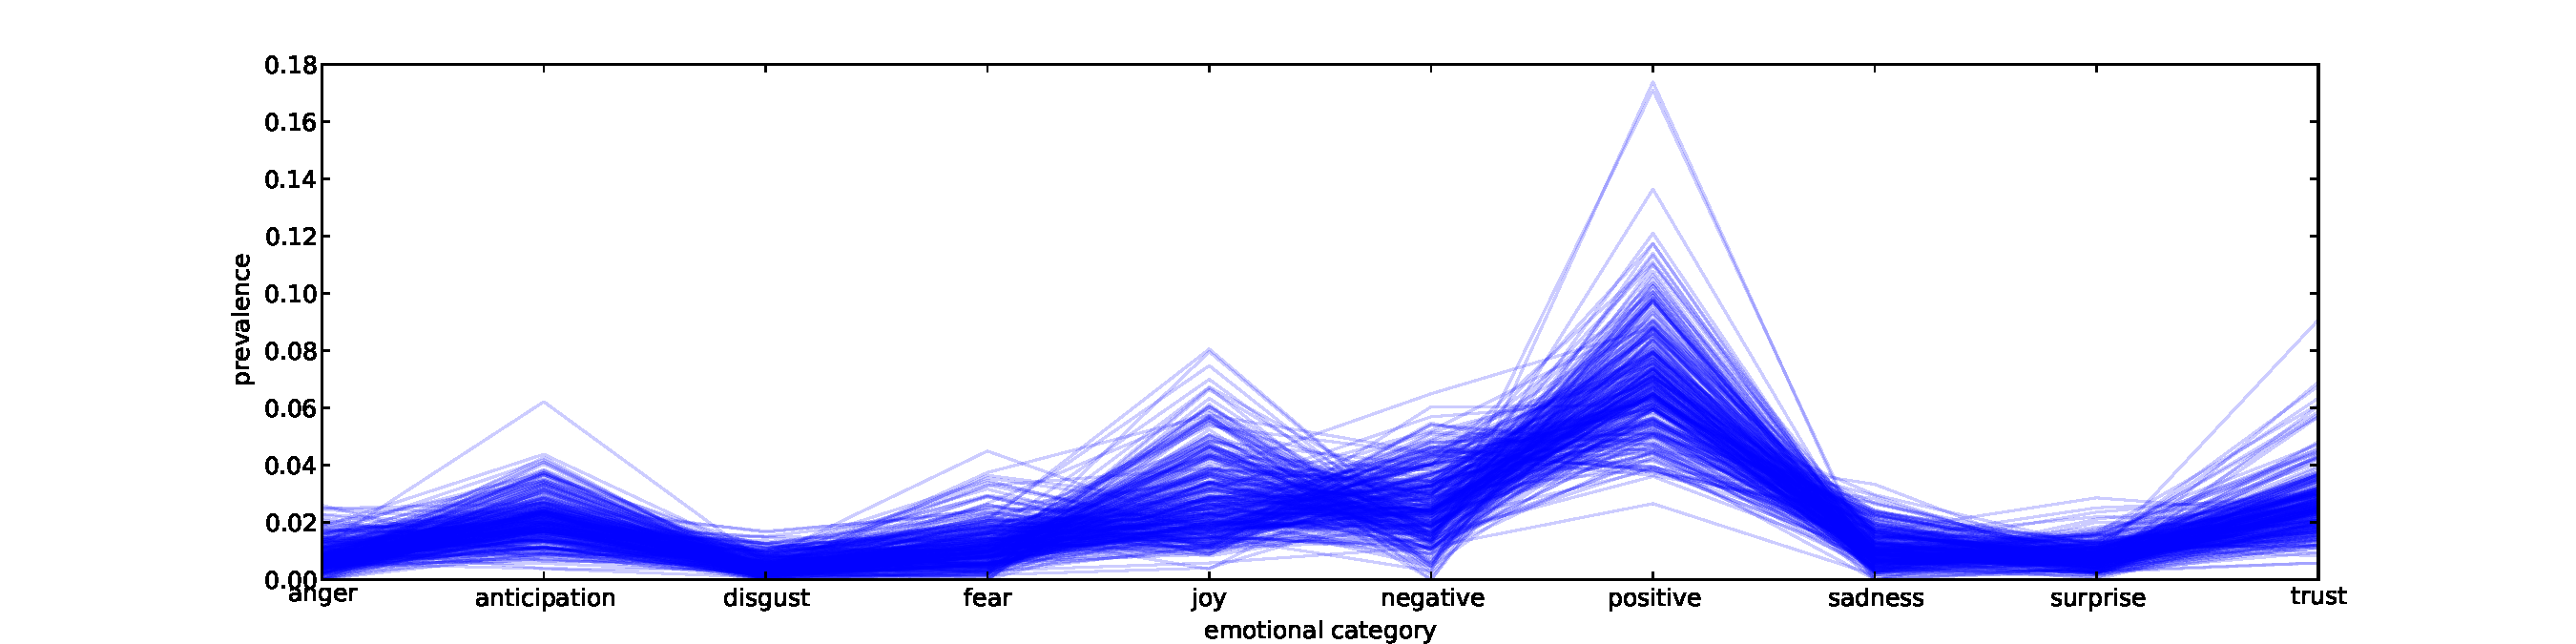
\includegraphics[scale=0.4]{../experiments/exp10.pdf}}
\end{align*}
\end{center}
\vspace{-.6cm}
\caption{A histogram of word distributions of the response for each poem. Here, each poem is represented by one line. The heavy overlap suggests that there is much similarity in the word distribution over comments.}
\vspace{.5cm}
\label{histogram}
\end{figure*}


\subsection{Predicting Proportion of Affect Words}
Next, we aim to characterize the magnitude of affect words in the user response. We describe this concept with the relative proportion of affect words. Multiple poetic features are correlated with the affect ratio, as shown in Table~\ref{feature-correlation}. Notably, the strongest correlated features with $p \le 0.005$ are: HGI-positiv, HGI-concrete, NRC-joy, NRC-trust, NRC-anticipation, type-token ratio, perfect rhyme score, and proportion of stops. %%TODO : Rob--this would be a good lead-in into what you will mention in the discussion... why do our results seem counter-intuitive after Kao's?
 When using such features, we are able to predict the affect ratio with 34.6\% reduction in error over simply predicting the average.

\begin{figure*}[ht]
\begin{center}
\begin{align*}
\centerline{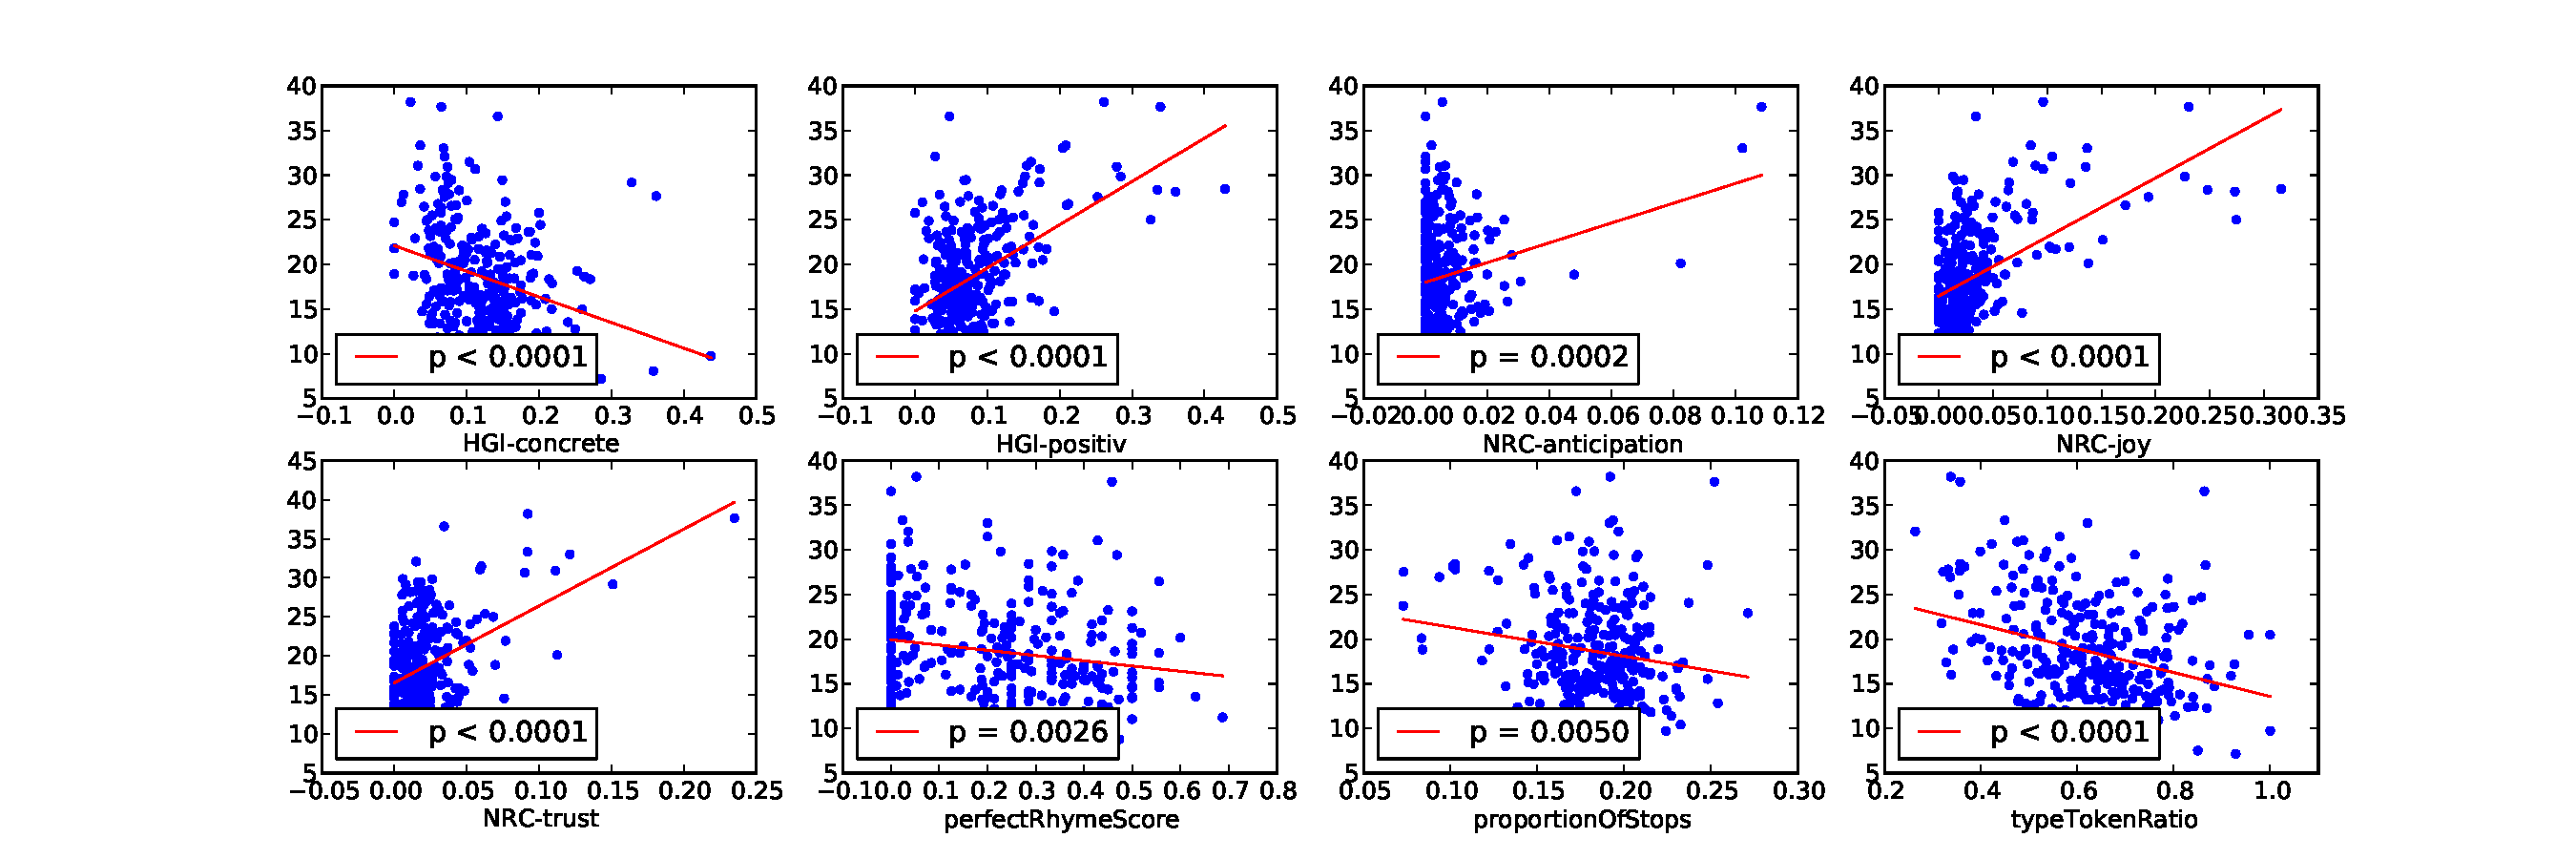
\includegraphics[scale=0.4]{../experiments/affect-ratio.pdf}}
\end{align*}
\end{center}
\vspace{-0.8cm}
\caption{A collection of scatter plots showing the correlation of the poem features and the comment affect ratio.}
\vspace{0.5cm}
\label{affect-ratio-features}
\end{figure*}


\begin{table*}['ht]
\scriptsize
\begin{center}
\label{feature-correlation}
\vskip 0.12in
\begin{tabular}{l @{\hspace{15pt}} rr @{\hspace{20pt}} rr @{\hspace{20pt}} rr @{\hspace{20pt}} rr @{\hspace{20pt}} rr}
\toprule[.12em]\addlinespace
&\multicolumn{2}{c}{Affect ratio}&\multicolumn{2}{c}{Type-token ratio}&\multicolumn{2}{c}{Avg. comment len.}&\multicolumn{2}{c}{Rating}&\multicolumn{2}{c}{Num. comments}
\\ Feature & correl. & p & correl. & p & correl. & p & correl. & p & correl. & p
\\ \addlinespace \midrule \addlinespace
NRC-joy & $0.51$ & $<0.0001$ & -$0.39$ & $<0.0001$ & -$0.34$ & $<0.0001$ & $0.06$ & $0.1883$ & -$0.07$ & 0.2583
\\ HGI-positiv & $0.51$ & $<0.0001$ & -$0.35$ & $<0.0001$ & -$0.31$ & $<0.0001$ & $0.07$ & $0.1531$ & -$0.10$ & 0.1013
\\ NRC-trust & $0.42$ & $<0.0001$ & -$0.25$ & $<0.0001$ & -$0.29$ & $<0.0001$ & -$0.02$ & $0.6105$ & -$0.11$ & 0.0578
\\ type-token & -$0.32$ & $<0.0001$ & $0.24$ & $<0.0001$ & $0.23$ & $0.0001$ & -$0.14$ & $0.0019$ & $0.02$ & 0.7834
\\ HGI-concrete & -$0.30$ & $<0.0001$ & $0.12$ & $0.0395$ & $0.14$ & $0.0189$ & -$0.07$ & $0.1130$ & $0.01$ & 0.8386
\\ NRC-anticipation & $0.22$ & $0.0002$ & -$0.09$ & $0.1223$ & -$0.15$ & $0.0109$ & -$0.01$ & $0.8357$ & -$0.08$ & 0.1523
\\ perfect rhyme score & -$0.18$ & $0.0026$ & $0.16$ & $0.0075$ & $0.16$ & $0.0080$ & -$0.05$ & $0.3116$ & -$0.09$ & 0.1171
\\ proportion of stops & -$0.16$ & $0.0050$ & $0.18$ & $0.0026$ & $0.18$ & $0.0021$ & $0.03$ & $0.4866$ & $0.11$ & 0.0594
\\ \addlinespace\bottomrule[.12em]
\end{tabular}
\caption{Features most strongly correlated with affect ratio.}
\end{center}
\end{table*}

\subsection{Predicting Average Response Length}
Clearly, there is an identifiable difference in the text of the responses. With the goal of further clarifying this difference, we attempt to predict the average response length. Using the same features as above, we are able to predict this with 15.7\% reduction in error over guessing the average. As observable in Table~\ref{feature-correlation}, the features’ correlations with average response length was the opposite of their correlation with average response length. That is, for example, though increased type-token ratio in the poem was correlated with decreased affect ratio, it was also correlated with \emph{increased} comment response length.

\subsection{Predicting Type-Token Ratio}
Additionally, we attempted to predict the type-token ratio of the responses given the poetic features identified as most useful in predicting affect ratio. Feature correlations with type-token ratio were similar to those with average response length, as shown in Table~\ref{feature-correlation}. That is, for example, poem type-token was positively correlated with both average response length and comment type-token ratio. We were able to predict type-token ratio with 17.0\% reduction in error over guessing the average.

\subsection{Predicting Average Rating}
\newcite{kao2012computational} suggest that poem aesthetics can be captured using poetic features. Using public approval as a mark of aesthetic value, one should be able to predict the average poem score using our features. However, we were unable to predict this feature well. This is also expected from Table~\ref{feature-correlation}, which shows that features for this metric did not have both high correlation and low p-value, which holds even for the omitted features.

\subsection{Predicting Number of Comments}
Similarly, one might use the number of comments as a mark of aesthetic value. Increased number of comments could be seen as a mark of increased popularity, or of engendering more discussion. However, we were unable to predict this either.

\section{Discussion and Error Analysis}
In this paper, we drew upon earlier computational work in the analysis of poetry to develop a set of linguistic and poetic features which we then used in a series of classification tasks aimed at predicting the \emph{emotional} content of responses for a given poem. While predicting emotional word-association distributions proved to be a dead end, we achieved interesting results in predicting the magnitude of \emph{affect} words, type-token ratio, and emotional ``intensity'' %TODO : [did we do this?]
 of the words in the comments for a given poem.

In particular, considering the features that proved to have a statistically significant impact in our prediction tasks, we found that more highly emotive poems tend to have %TODO : [significant features list].

These results were surprising to a certain extent, not in the least because at first glance they appear to contradict \newcite{kao2012computational}. In their work, Kao and Jurafsky found that %%TODO [stat significant features etc]
 were indicators of poetry written by professionals, as compared with poetry written by amateurs. One might assume that professional poetry is far more likely to be effective at producing an emotive response, so to find that within our dataset of professional poetry opposite trends produced more \emph{emotive} poetry per our metrics is a finding that requires a further explanation.

Looking by hand at the sets of responses which we found to have a high proportion of affect words, we notice a large contrast between commentary having high affect ratio and commentary having high affect ratio:

\begin{itemize}
\item \emph{what beautiful use of words. lovely poem.}
\item \emph{you two are a couple of losers.}
\end{itemize}

contrasted with comments having low affect ratio:

\begin{itemize}
\item \emph{christ's life is plausible. however, consider the theme of ambition: what it is; whether it is neutral or with the power to possess good or evil; and its source. then think to how 'we people on the pavement' took to a person whose skeletons were not on public display.}
\item \emph{this is poetic therapy at its very best. life-changing and liberating. i can't stop reading it...}
\end{itemize}

Indeed, the high aspect ratio comments tended to be very short ones, as shown in Figure~\ref{affect-ratio-length}. Further examination shows that affect ratio, log of average comment length, and comment type-token ratio are all strongly correlated with each other. We can offer an interpretation: some comments are very short and offer praise (or critique, as shown above) without explanations, and other comments are lengthy and detailed. 

\begin{figure*}[ht]
\begin{center}
\begin{align*}
\centerline{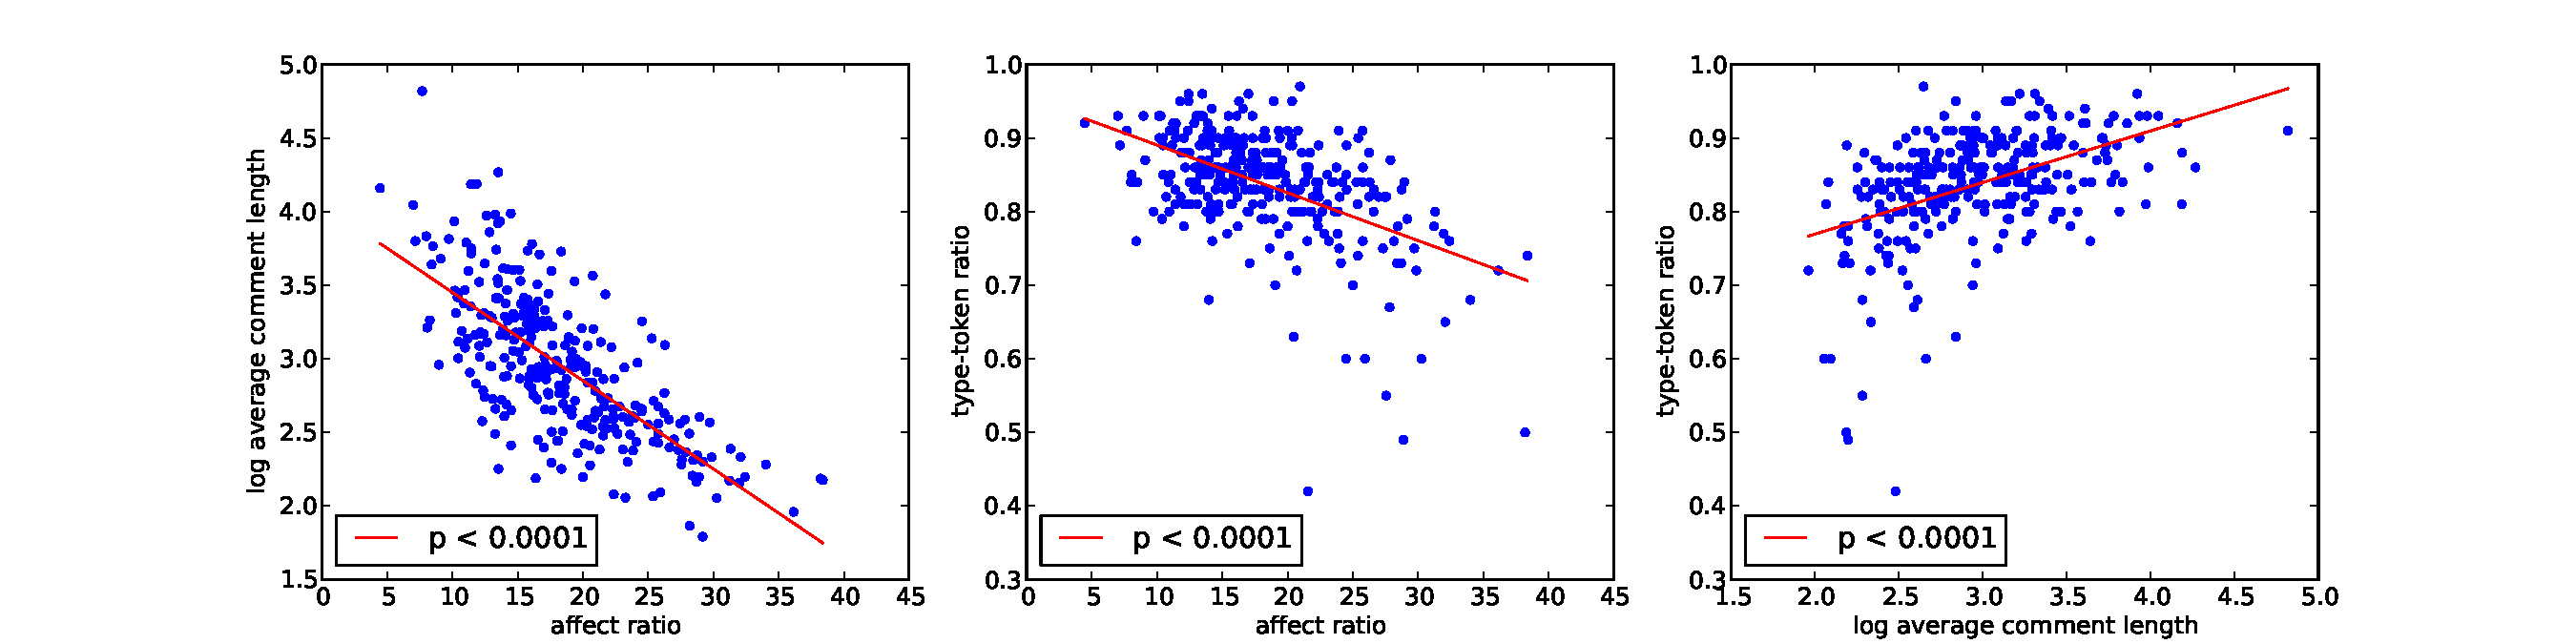
\includegraphics[scale=0.4]{../experiments/exp12.pdf}}
\end{align*}
\end{center}
\caption{A collection of scatter plots showing the correlations of affect ratio, log average comment length, and comment type-token ratio.}
\label{affect-ratio-length}
\end{figure*}

justification / explanation of phonetic features: 
   Holland quote to use --- ``in poetic language, \dots particular sounds involve muscular actions that somehow match the sense.'' \cite{holland1989dynamics}.


\section{Future work}



\section*{Acknowledgments}

Do not number the acknowledgment section. Do not include this section when submitting your paper for review.


\bibliographystyle{acl}
\bibliography{bib}


\end{document}


